O mesmo aparato de caracterização de conjuntos de dados foi testado em outras modalidades de recomendação automática, como segue:
\begin{itemize}
   \item predição da melhor estratégia para um dado algoritmo de aprendizado (Seção \ref{recest});
   \item predição do melhor par estratégia-algoritmo (Seção \ref{recpar});
   \item predição da melhor métrica para estratégias baseadas em distância (Seção \ref{recdist}); e,
   \item recomendação sobre a aplicação ou não de aprendizado ativo (Seção \ref{reccon}).
\end{itemize}
De todas essas possibilidades testadas, a recomendação de estratégias e de pares mostraram-se as modalidades mais promissoras.

\subsection{Recomendação de estratégias}\label{recest}
% poucas strats pode ser bom, mas um número pequeno demais faz com que o valor de correlação de ranking seja com pouco significado.
Uma investigação inicial sobre a possibilidade da recomendação automática de estratégias de amostragem ativa, dado um algoritmo de aprendizado, foi realizada.
Trata-se de uma abordagem, de certa forma, complementar à contemplada na Seção \ref{recalg}.
% Sem prejuizo das análises posteriores,

O conjunto de estratégias foi arbitrariamente reduzido para o seguinte, visando uma quantidade reduzida de metaclasses, mas representando as diferentes abordagens estudadas: EERent, HS e HTUeuc.
Considerou-se que as estratégias baseadas em densidade ou incerteza foram representadas por HTUeuc e as estratégias agnósticas por HS.
A ausência de aprendiz da estratégia HS e seu peculiar viés de exploração colaboram para a diversidade do conjunto.


Os valores de correlação média entre os ranqueamentos preditos e os esperados são apresentados na Figura \ref{stcorr}.
\begin{figure}
\centering
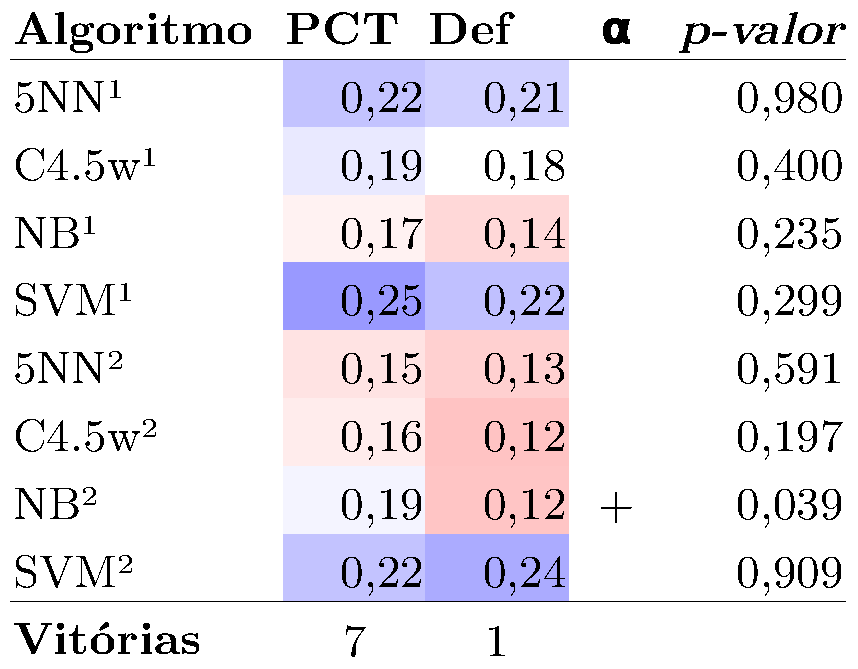
\includegraphics[scale=0.4]{images/metastcorr.pdf}
\caption[Comparação da correlação na predição de ranqueamento de estratégias.]{Comparação do coeficiente de correlação de Spearman na predição de ranqueamento de estratégias.
\textit{Detalhes na Figura \ref{alcmeta}.}}
\label{stcorr}
\end{figure}
De acordo com esses resultados, PCT superou Def com significância estatística na predição de ranqueamentos somente para o algoritmo NB, durante a segunda metade do período de aprendizado (2 sobrescrito).
Entretanto, por situar-se entre múltiplas comparações, essa vantagem isolada pode ser resultado do acaso devido à possibilidade de ocorrência do erro de tipo I global \cite{journals/jmlr/Demsar06}. % family-wise error
Logo, embora superior numericamente em sete casos, não é possível afirmar com significância estatística, diante desses resultados, que o meta-aprendizado tenha sido vantajoso.
O sucesso da proposta, assim, é menos evidente do que na Figura \ref{corrmeta}, apresentada previamente, correspondente à recomendação de algoritmos.

A viabilidade da recomendação de estratégias é mais clara na tarefa de predição de metaclasses - conforme ilustrado na Figura \ref{stkap}.
\begin{figure}
\centering
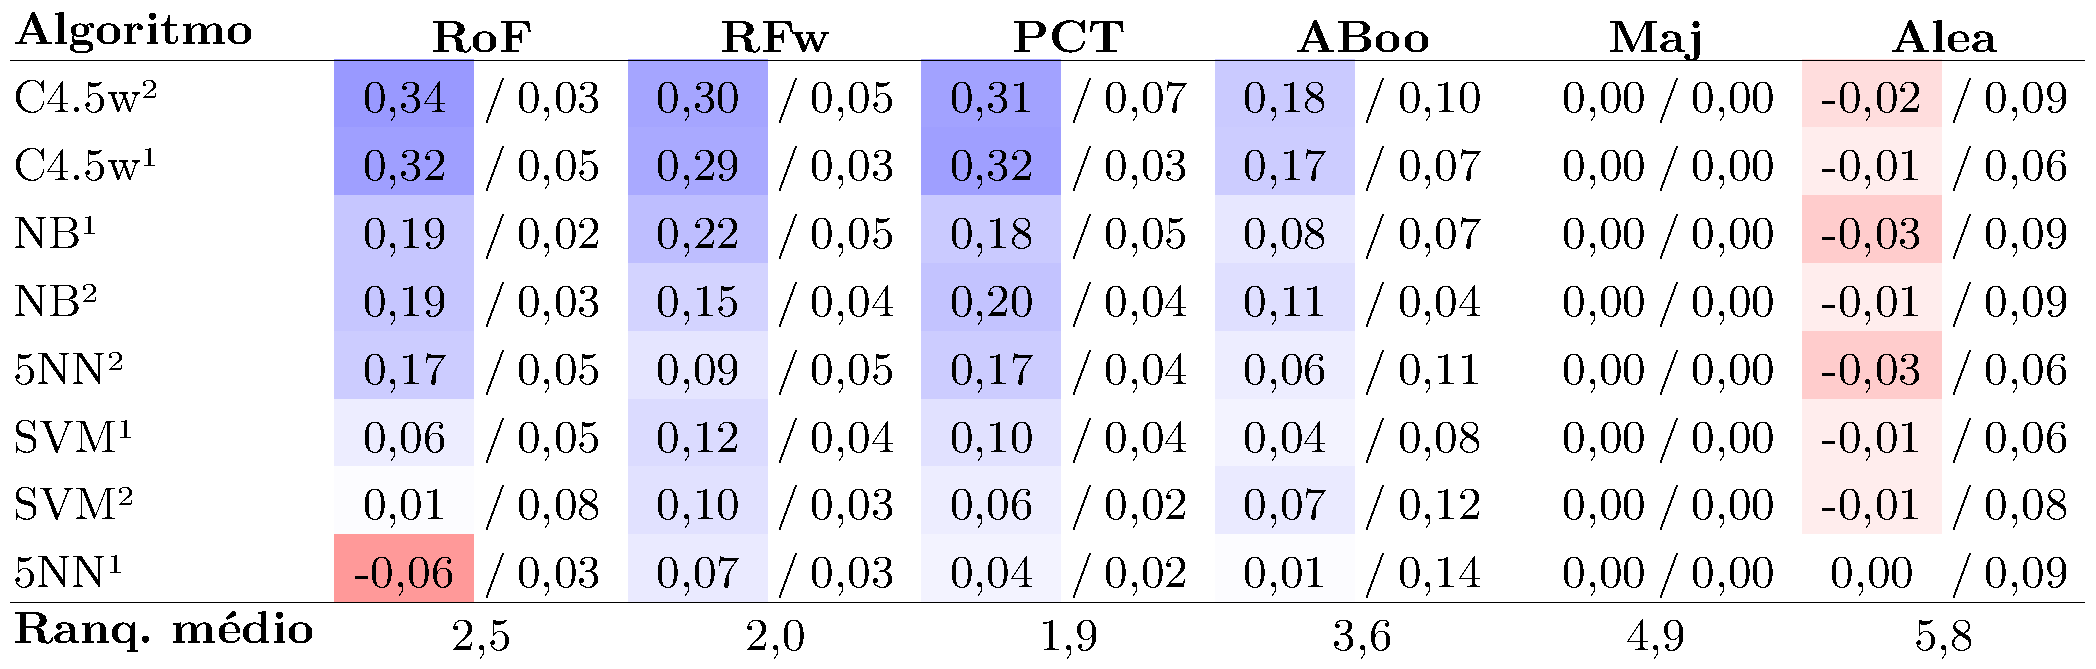
\includegraphics[scale=0.4]{images/metastkap.pdf}
\caption[Comparação de $\kappa$ na recomendação da melhor estratégia.]{Comparação de $\kappa$ (média/desvio padrão) na recomendação da melhor estratégia.
\textit{Detalhes na Figura \ref{accmeta}.}}
\label{stkap}
\end{figure}
Os meta-aprendizes obtiveram desempenho inferior à referência ($\kappa=0$) em apenas um caso.
PCT atingiu a melhor colocação média dentre os quatro meta-aprendizes considerados.
Porém, um aspecto negativo nesses resultados é que os piores desempenhos preditivos no nível meta ocorreram com os algoritmos de maior destaque no nível base: SVM e 5NN.
Isso significa que o nível meta pode ter um bom desempenho preditivo para algoritmos possivelmente inadequados - reduzindo a utilidade prática da metaestratégia.
Apesar disso, de acordo com os resultados apresentados e consideradas as limitações do aparato experimental adotado, pode-se dizer que \destaque{a recomendação de estratégias de amostragem ativa é promissora}\footnote{Desde que a coleção contenha mais do que um conjunto de um mesmo domínio (conforme demonstrado posteriormente no Apêndice \ref{apflu})}, embora represente um maior desafio que a recomendação de algoritmos.

\subsection{Recomendação de pares estratégia-algoritmo}\label{recpar}
Um desdobramento natural da investigação realizada nas seções anteriores
é a recomendação automática de pares estratégia-algoritmo.
Considerando os quatro algoritmos do nível base e as três estratégias adotadas como opções na recomendação de estratégias, tem-se um total de doze pares possíveis.
Apesar dessa grande quantidade de metaclasses, o meta-aprendiz foi capaz de superar Def na predição de ranqueamento de pares nas duas metades da curva de aprendizado com $\alpha=0,01$.
Isso pode ser visto nas duas linhas contendo os termos \textit{Todos os pares} na Figura \ref{parcorr}.
\begin{figure}
\centering
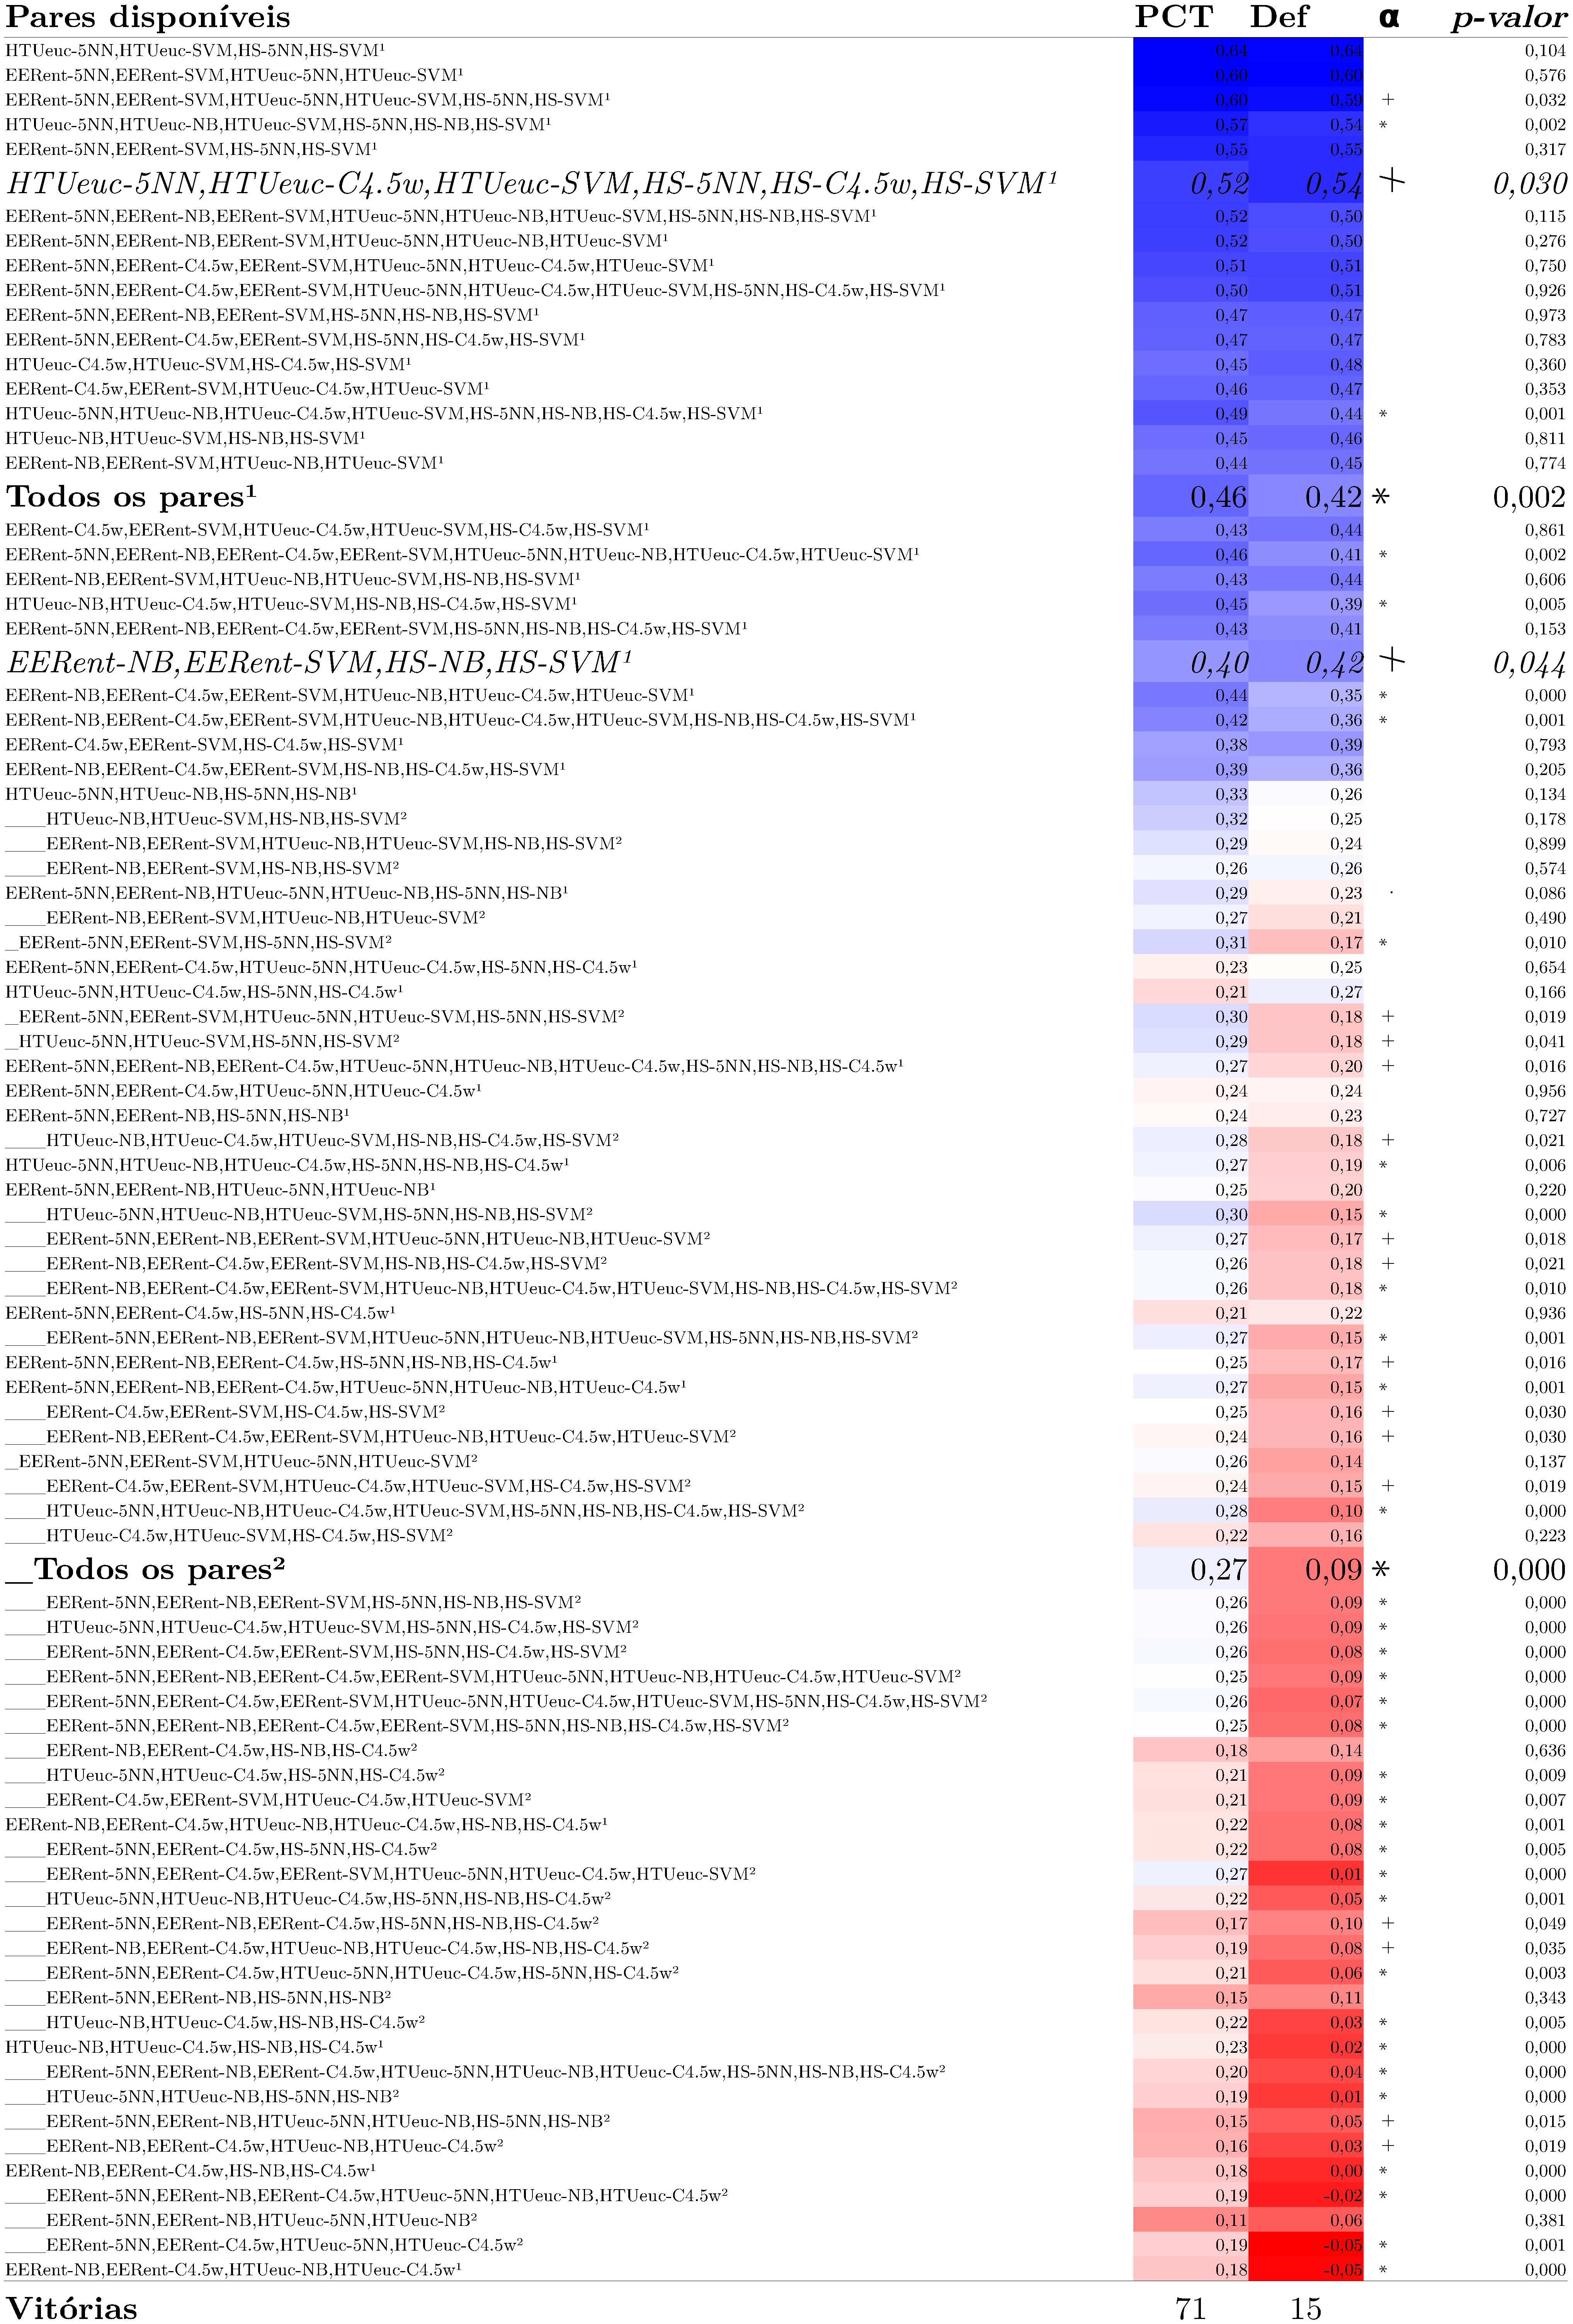
\includegraphics[scale=0.21]{images/metaparcorr.pdf}
\caption[Comparação da correlação, predição: ranqueamento estratégia-algoritmo.]{Comparação do coeficiente de correlação de Spearman na predição de ranqueamento de pares estratégia-algoritmo.
\textit{Linhas grafadas em itálico indicam diferença com significância estatística a favor do método de referência.}
\textit{Detalhes na Figura \ref{accmeta}.}}
\label{parcorr}
\end{figure}

As demais linhas representam experimentos em que todos os outros subconjuntos possíveis contendo pelo menos dois algoritmos e duas estratégias foram disponibilizados para o sistema de recomendação.
As linhas correspondentes à segunda metade do período de consultas estão deslocadas para a direita visando compensar a baixa legibilidade dos números sobrescritos.

% Quando consideradas apenas as combinações formadas pelos algoritmos de maior destaque (5NN e SVM), metade dos oito experimentos não apresentaram diferenças com significância estatística.
O meta-aprendiz PCT obteve um bom desempenho geral, sendo superior à referência 71 vezes contra 15; a maioria delas com diferenças estatisticamente significativas.
Portanto, no contexto do experimento, é possível afirmar que \destaque{a recomendação automática de pares estratégia-algoritmo é, no mínimo, promissora}\footnote{Desde que a coleção contenha mais do que um conjunto de um mesmo domínio (conforme demonstrado posteriormente no Apêndice \ref{apflu})}.
Tal constatação é reforçada na tarefa de classificação, em que as colocações médias dos meta-aprendizes (2,1; 2,1; 2,4 e 3,3) superaram aquelas obtidas pelas referências (5,0 e 5,2) - conforme mostrado na Figura \ref{par}.
\begin{figure}
\centering
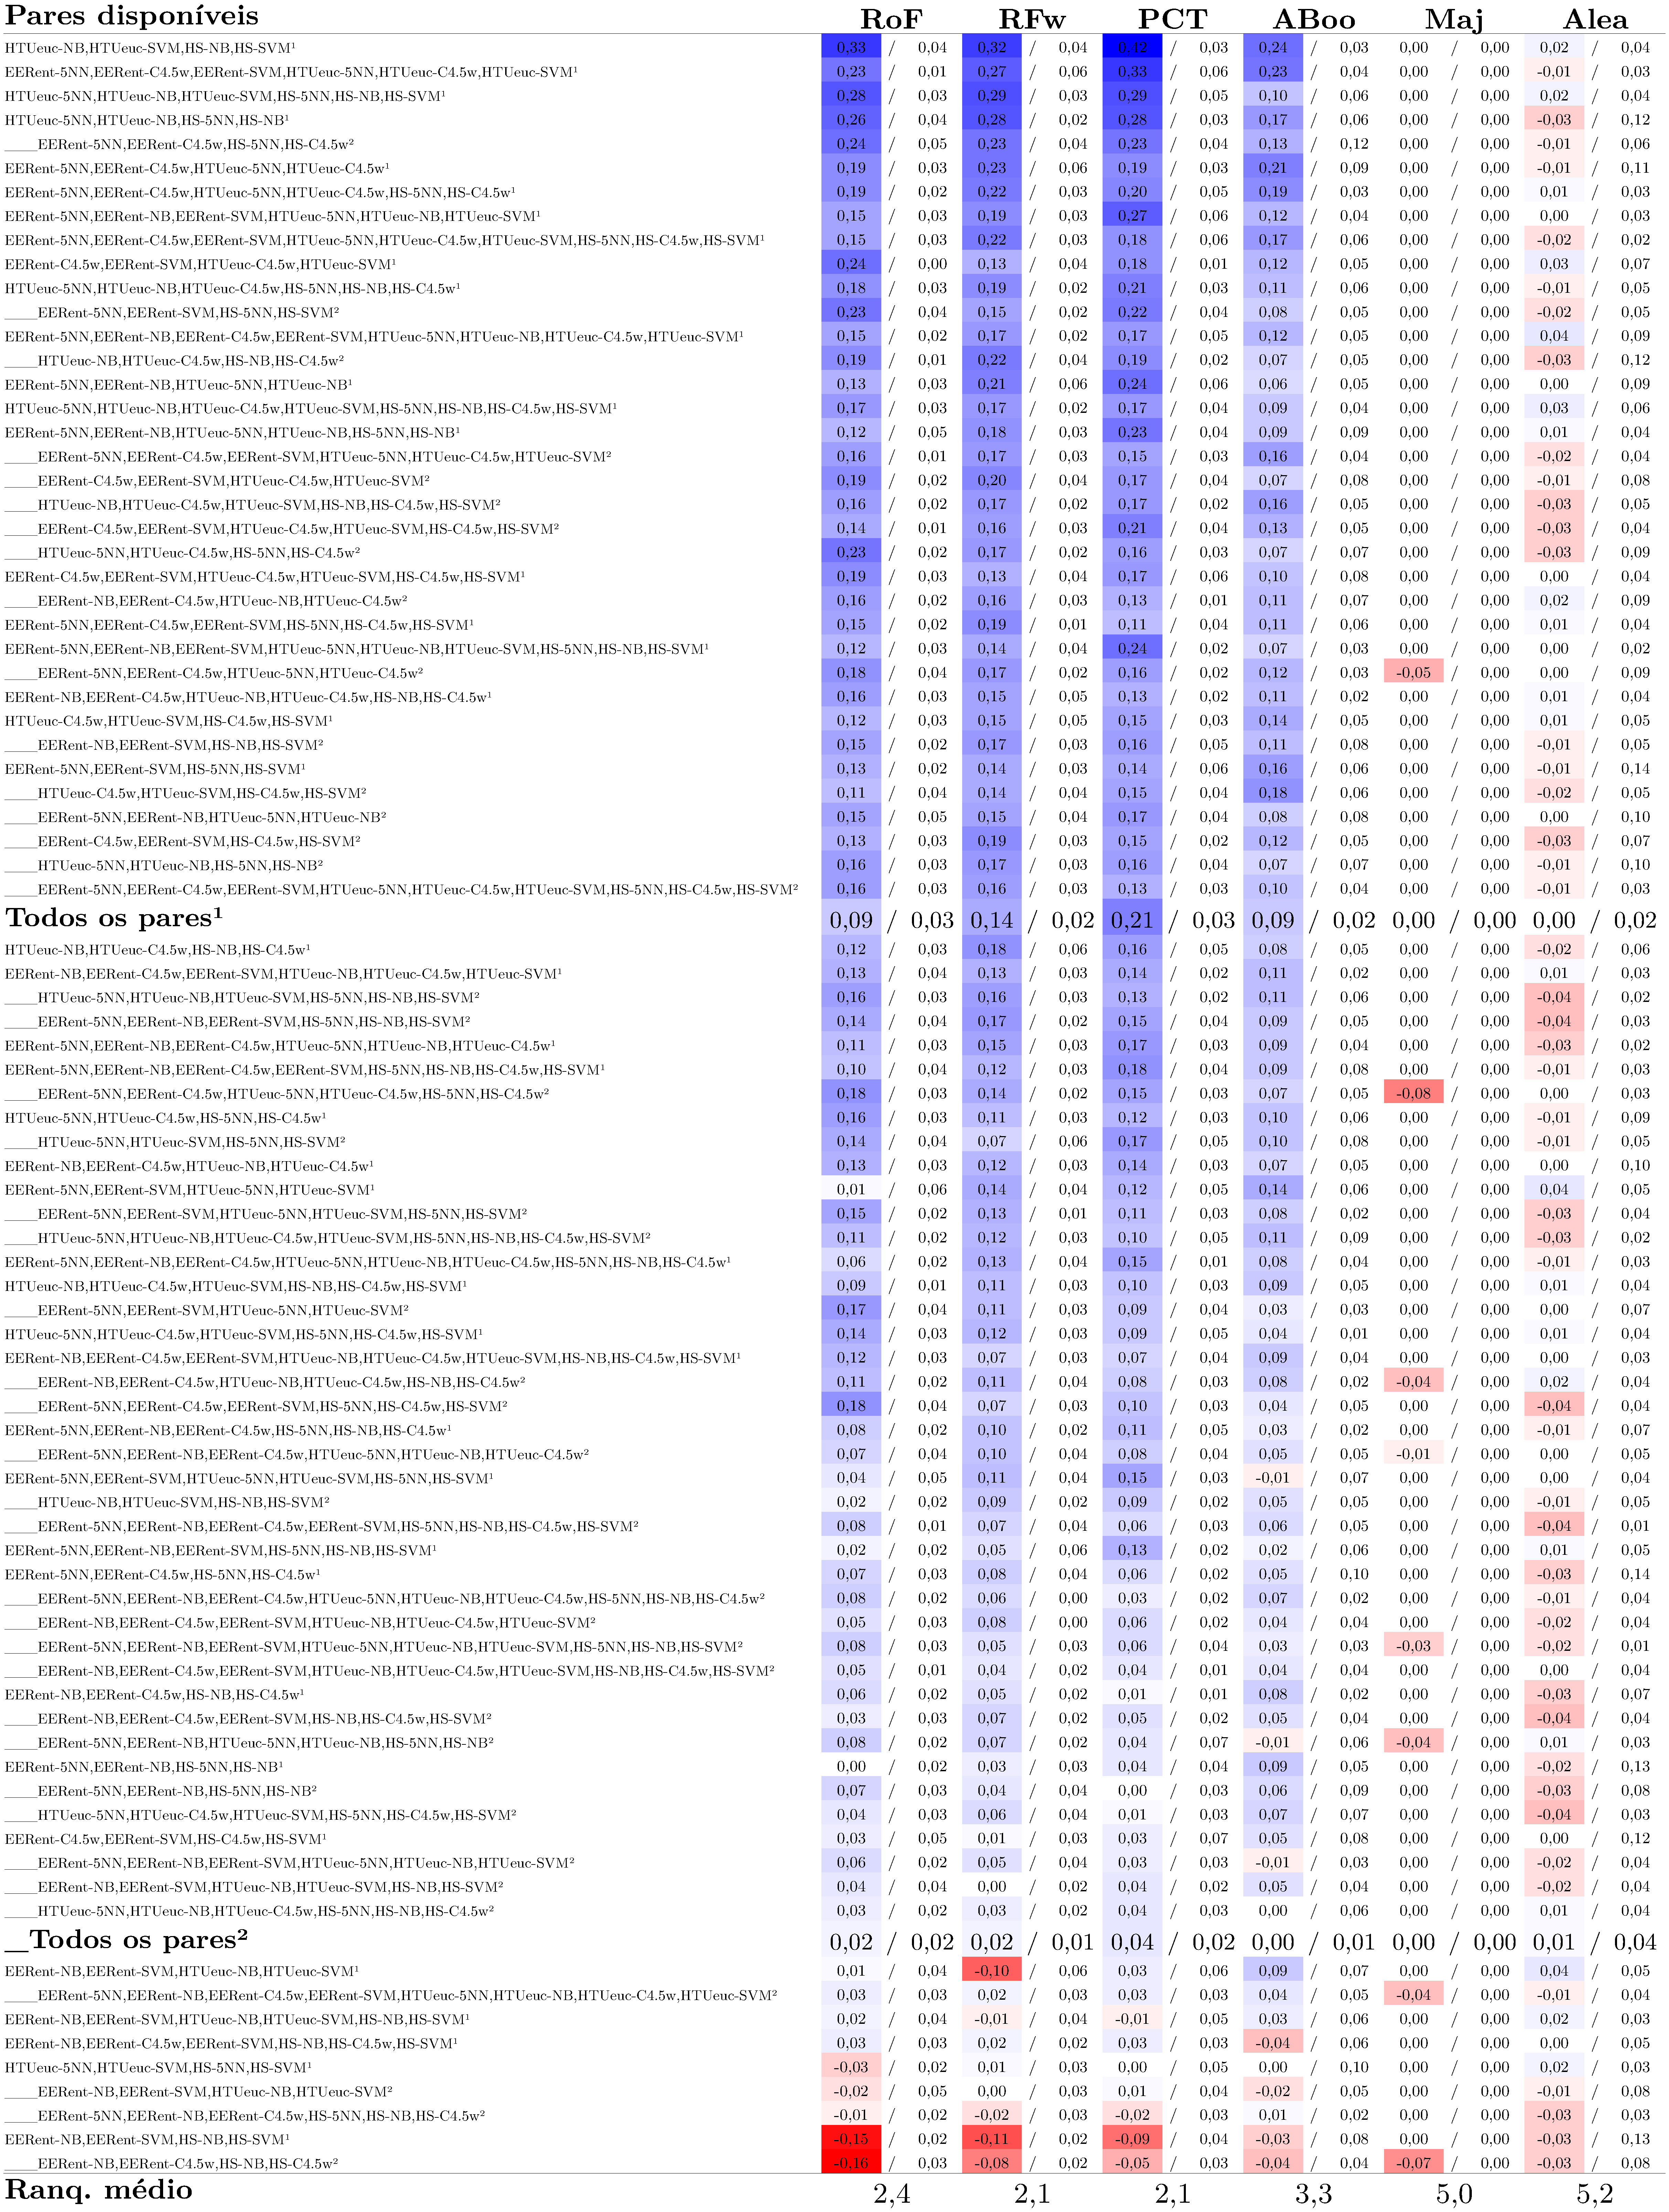
\includegraphics[scale=0.195]{images/metapar.pdf}
\caption[Comparação de $\kappa$ na recomendação do melhor par estratégia-algoritmo.]{Comparação de $\kappa$ (média/desvio padrão) na recomendação do melhor par estratégia-algoritmo.
\textit{Detalhes na Figura \ref{accmeta}.}}
\label{par}
\end{figure}
Nessa modalidade de meta-aprendizado, RFw e PCT compartilharam a segunda colocação, seguidos por RoF.

\subsection{Recomendação de métrica de distância}\label{recdist}
\simbolo{d_m(\bm{u},\bm{z})}{distância de Mahalanobis entre dois exemplos $\bm{u}$ e $\bm{z}$}
\simbolo{U}{matriz de exemplos da reserva}
\simbolo{\cov(U)}{matriz de covariância de $U$}

Um dos parâmetros que poderiam ser ajustados via meta-aprendizado é a métrica de distância das estratégias baseadas em densidade.
A distância de Mahalanobis foi acrescentada como opção \cite{mahalanobis1936generalized}, apesar de seu alto custo computacional ter levado à 
%reduzido a coleção, requerendo a 
exclusão dos seguintes conjuntos:
\textit{musk}, \textit{texture}, \textit{volcanoes-d1} e \textit{volcanoes-b5}.

Considerando cada exemplo da reserva $\bm{x}_i, 1 \leq i\leq |\mathcal{U}|$ como um vetor linha da matriz $U$, a distância de Mahalanobis $d_m$
% (\bm{u},\bm{z})$
entre dois exemplos $\bm{u}$ e $\bm{z}$ é baseada na matriz de covariância $\cov(U)$ - conforme as equações \ref{vetcols} e \ref{eqmaha}.
\begin{equation}\label{vetcols}
   U=\begin{pmatrix}
	\bm{x}_1 \\
	\bm{x}_2 \\
	\vdots \\
	\bm{x}_{|\mathcal{U}|}
	\end{pmatrix}
   \in \mathbb{R}^{|\mathcal{U}|\times|\mathcal{A}|}
\end{equation}
\begin{equation}\label{eqmaha}
	d_m(\bm{u},\bm{z})=\sqrt{(\bm{u} - \bm{z})^{\top} \cov(U)^{-1} (\bm{u} - \bm{z})}
\end{equation}
% The Mahalanobis distance is the same as the Euclidean distance if the covariance matrix is the identity matrix.

Cada par [estratégia baseada em densidade]-algoritmo foi representado por um experimento que consistia na recomendação automática de uma das três métricas de distância: euclidiana, Manhattan e Mahalanobis.
Os resultados contrariam a tendência promissora observada anteriormente nas outras modalidades de recomendação.
Na Figura \ref{distcorr}, Def obteve mais vitórias que PCT, algumas com significância estatística (sujeita ao erro de tipo I global).
\begin{figure}
\centering
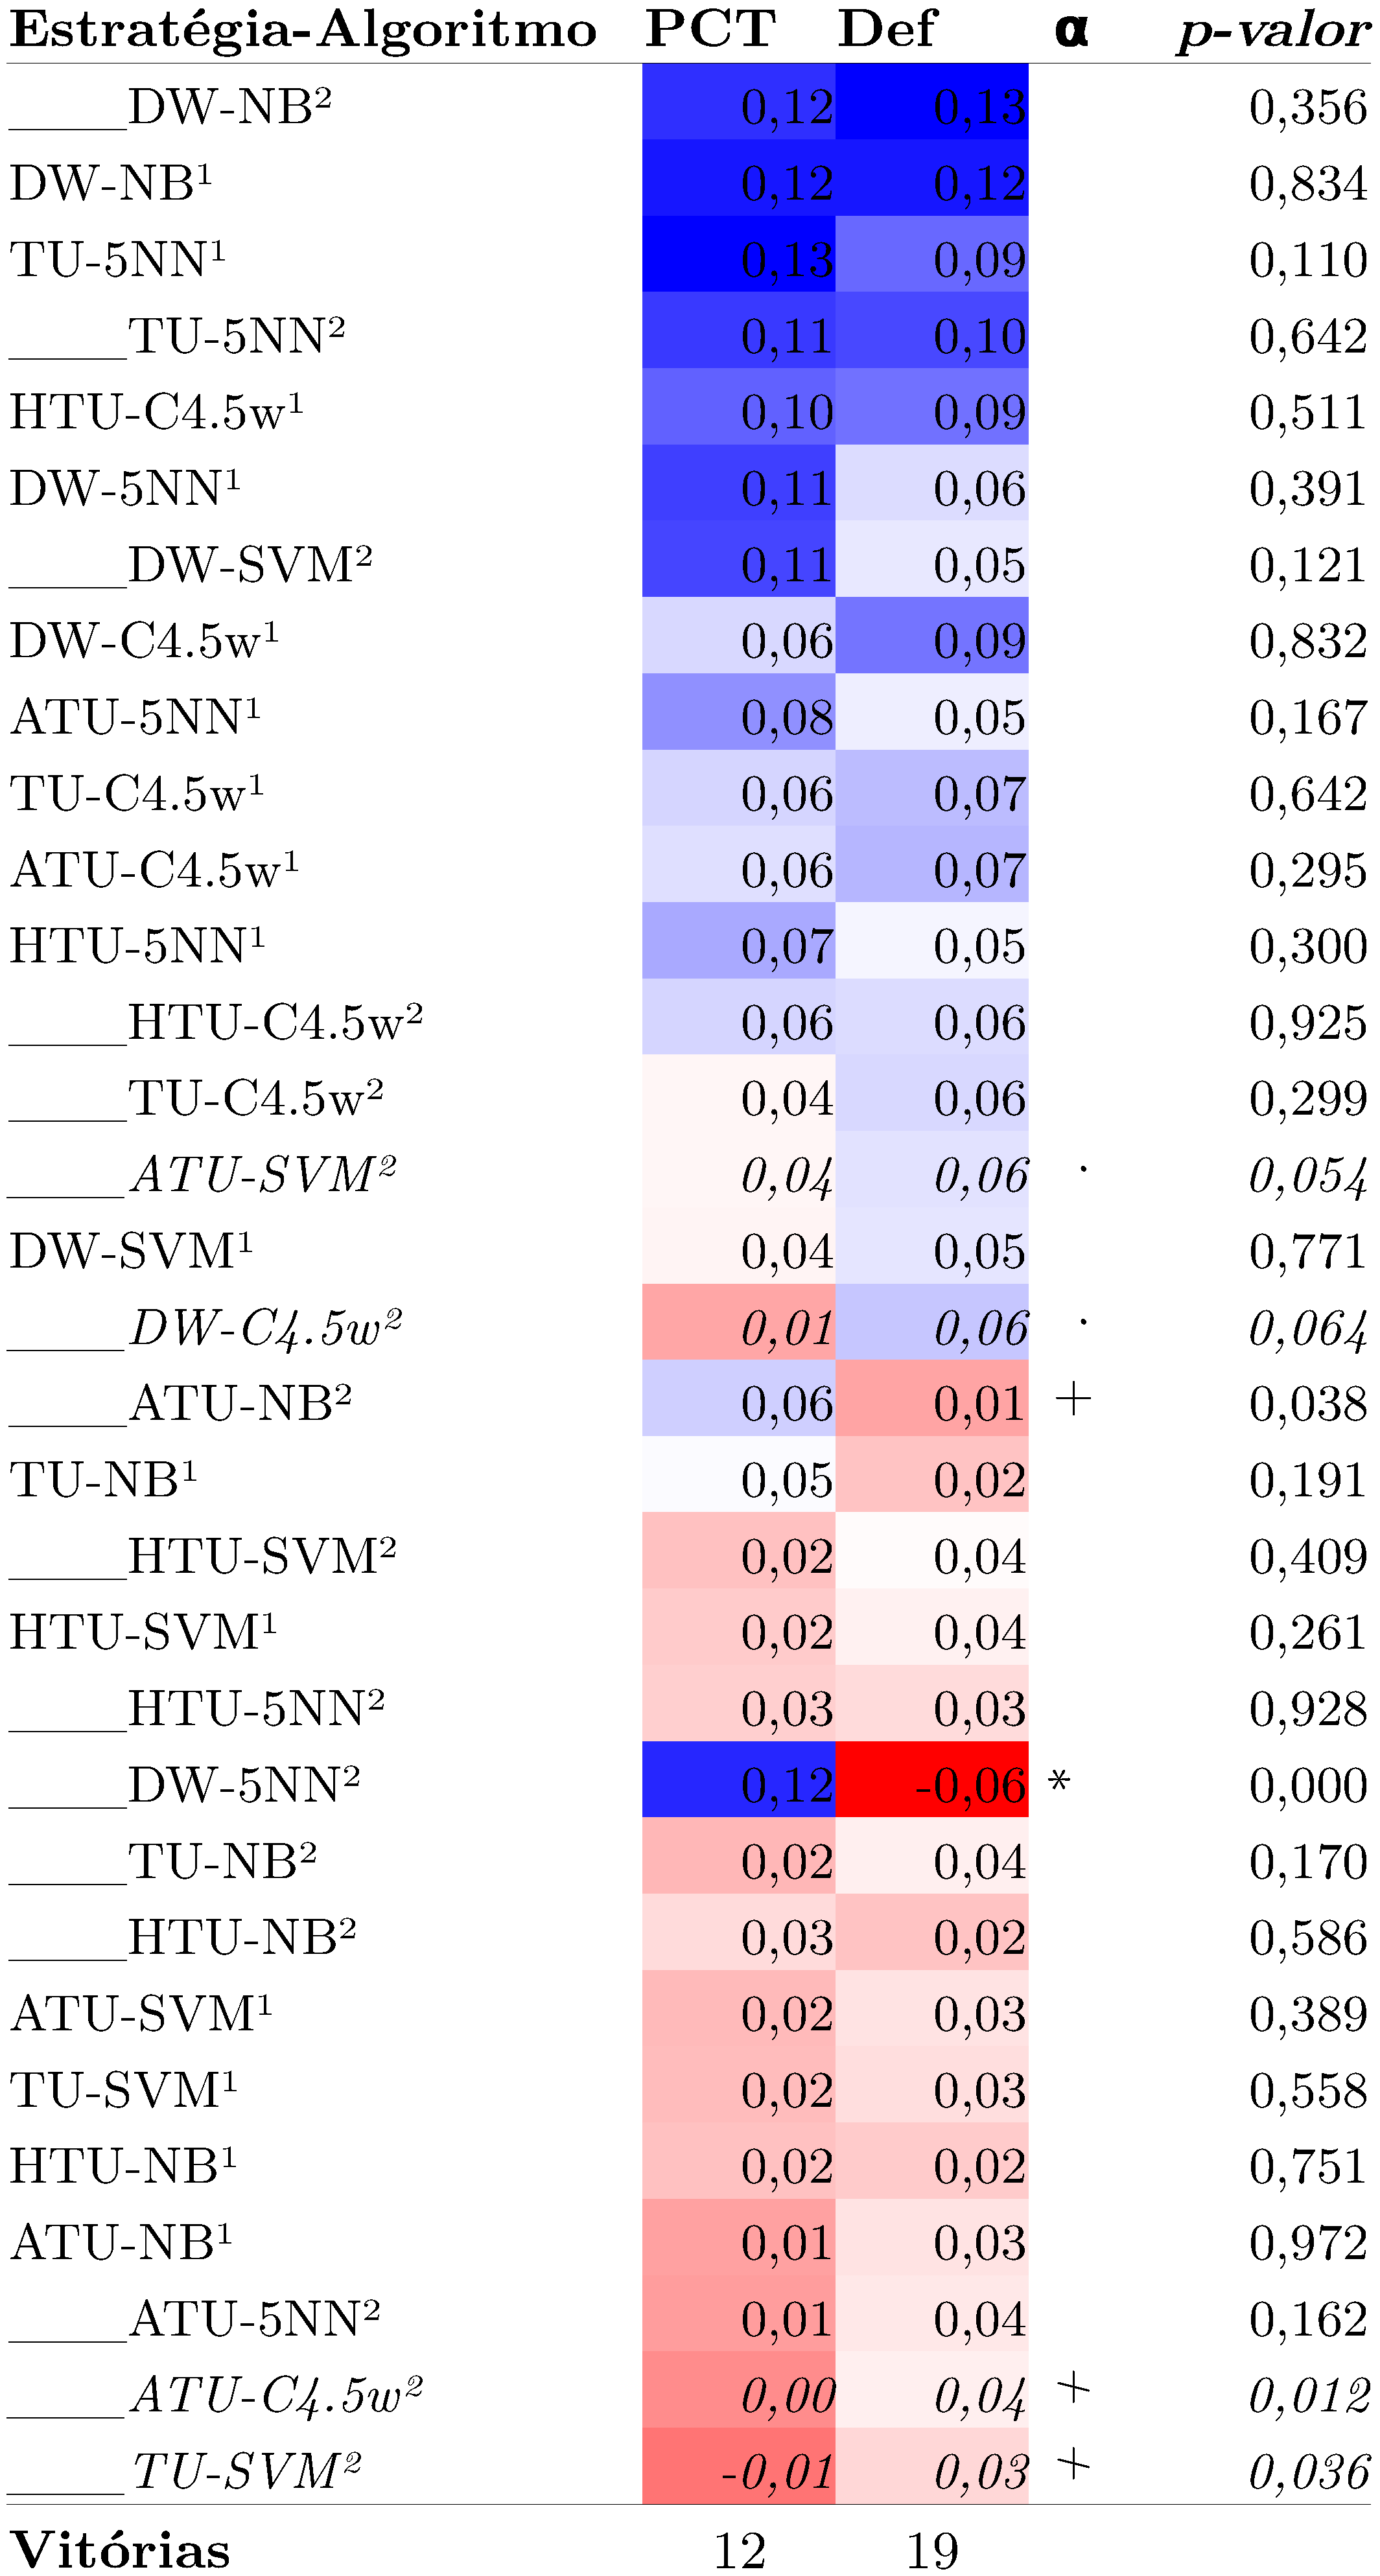
\includegraphics[scale=0.215]{images/metadistcorr.pdf}
\caption[Desempenho na predição de ranqueamento de medidas de distância.]{Desempenho na predição de ranqueamento de medidas de distância para estratégias baseadas em densidade.
\textit{Detalhes na Figura \ref{parcorr}.}}
\label{distcorr}
\end{figure}
Na predição de metaclasse, cujos resultados são apresentados na Figura \ref{dist}, a colocação média de todos os meta-aprendizes se situou próxima da colocação central (3,5), indicando que a escolha do algoritmo de aprendizado praticamente não influencia o resultado.
\begin{figure}
\centering
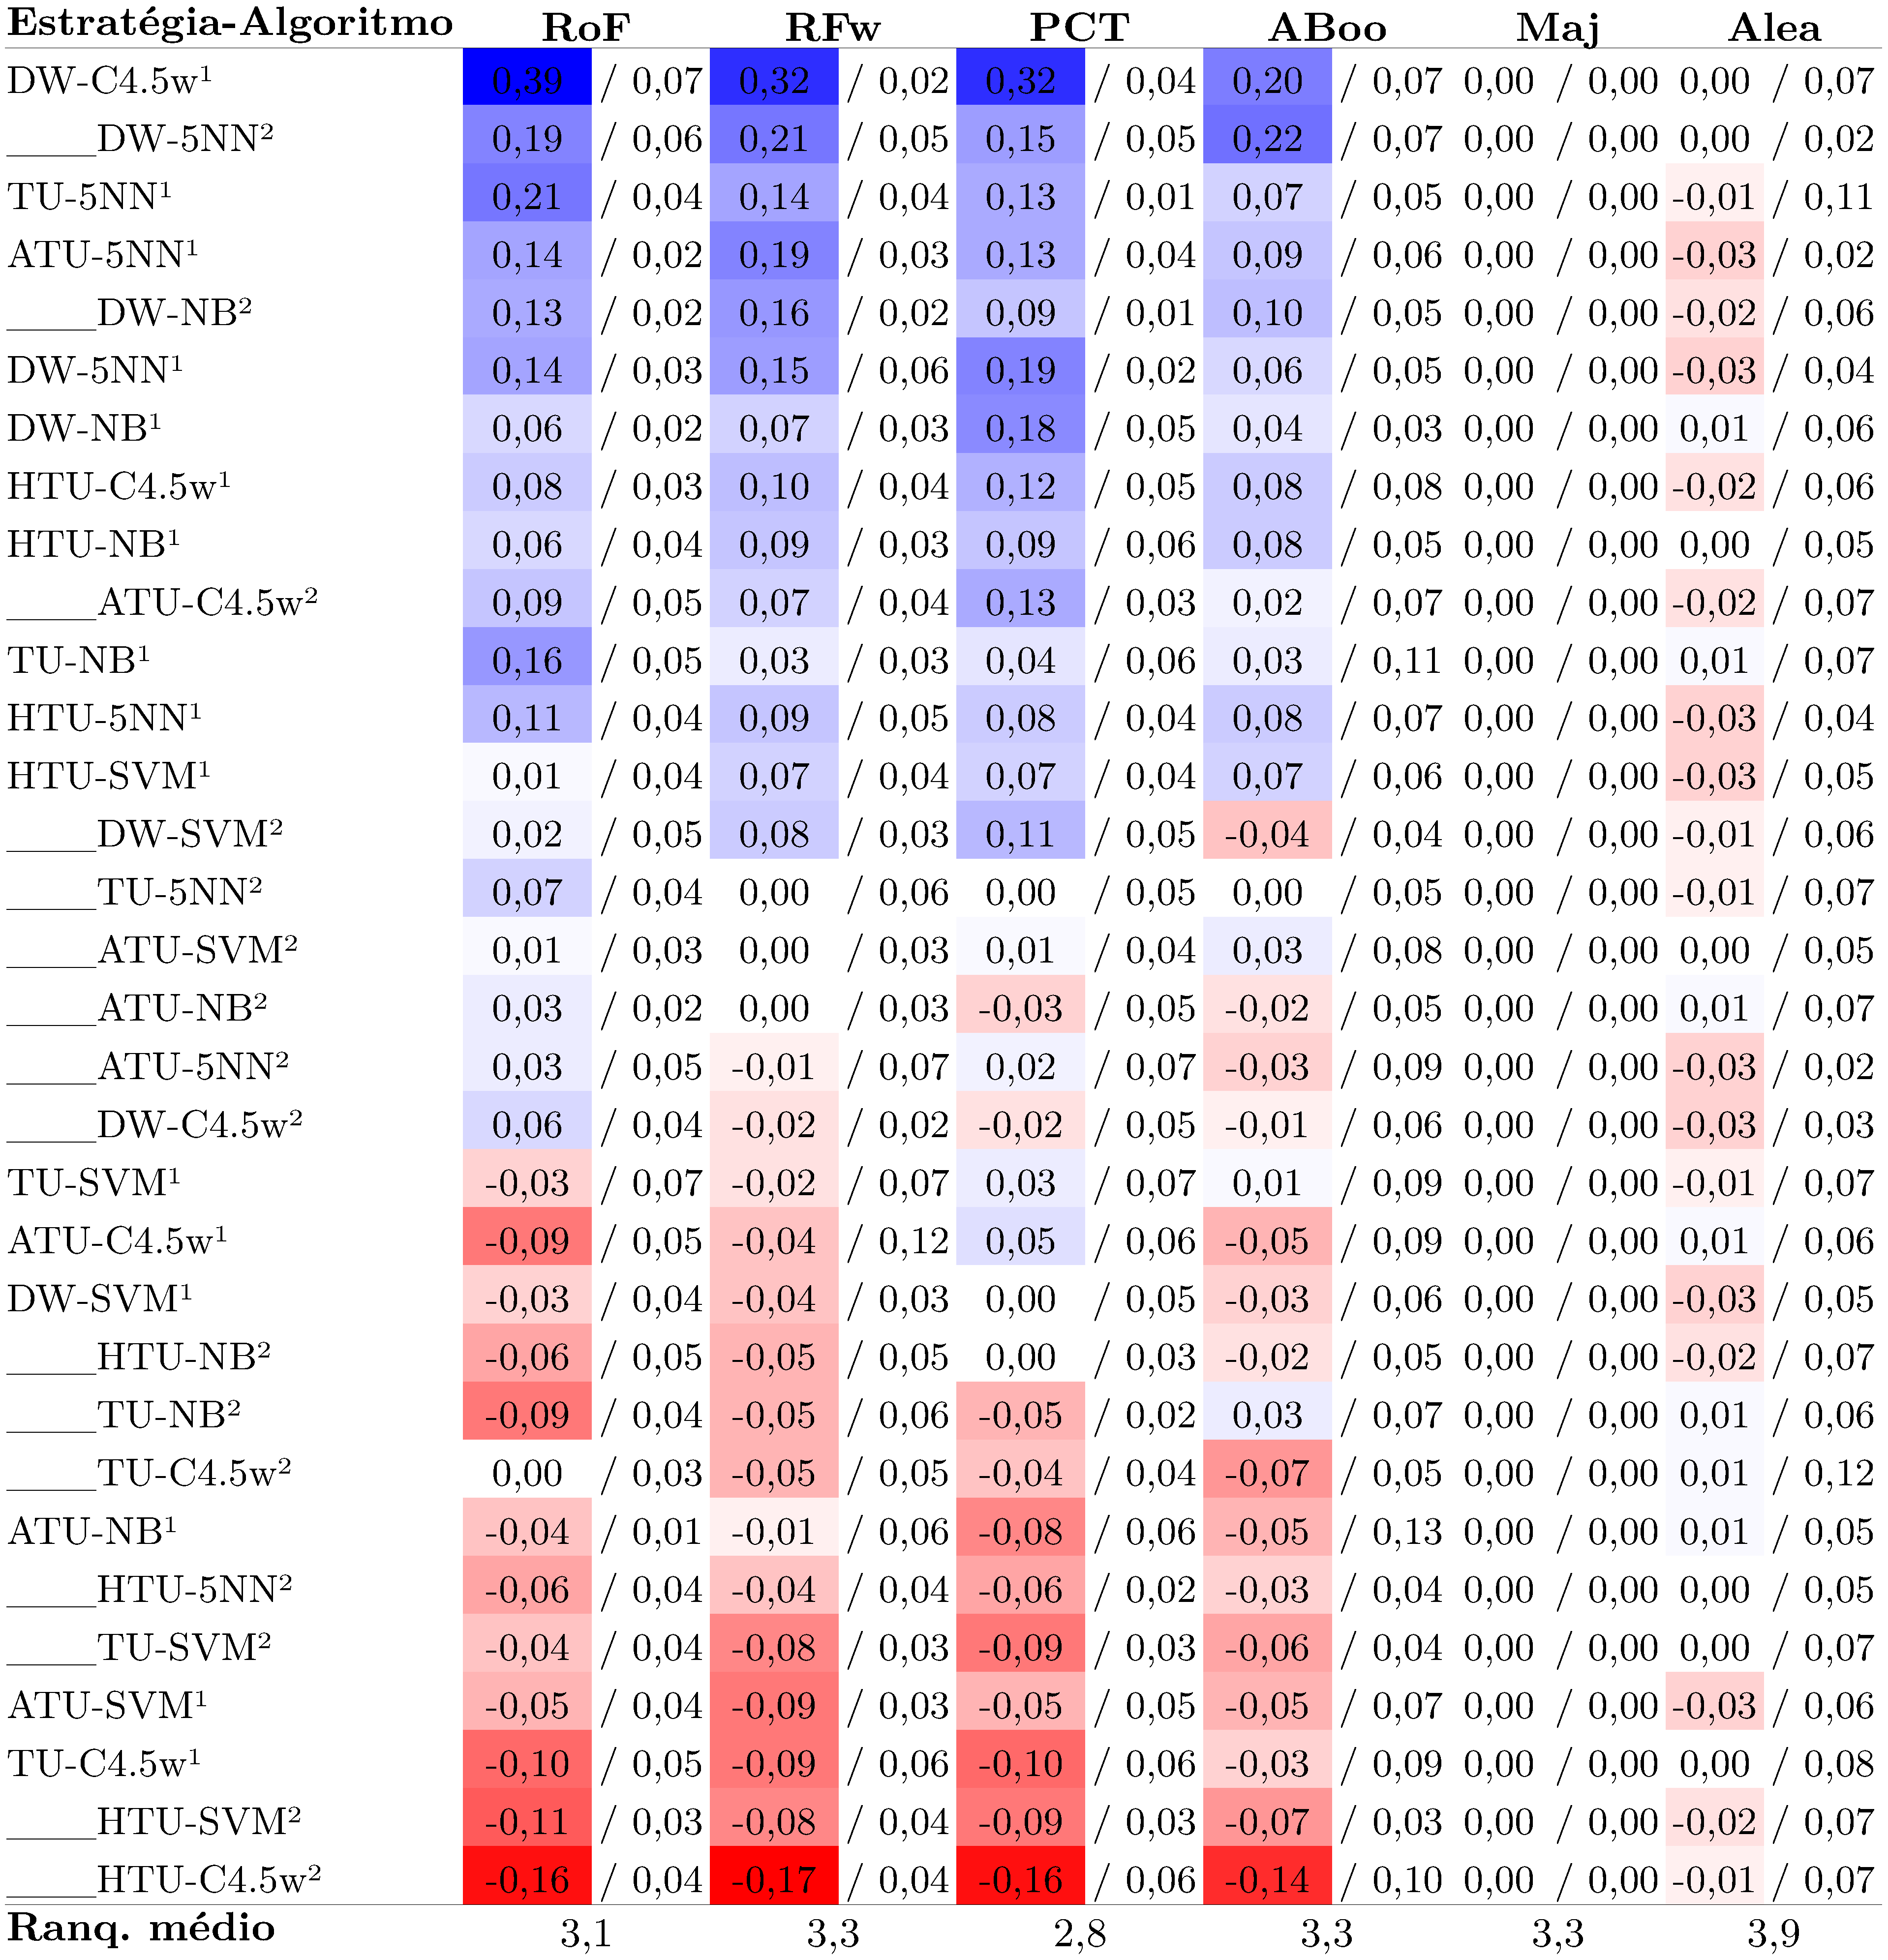
\includegraphics[scale=0.215]{images/metadist.pdf}
% acc: 10x10-fold
% teste: sem teste
\caption[Comparação de $\kappa$ na predição da melhor medida de distância.]{Comparação de $\kappa$ (média/desvio padrão) na predição da melhor medida de distância para estratégias baseadas em densidade.
\textit{Detalhes na Figura \ref{accmeta}.}}
\label{dist}
\end{figure}

Apesar de existir uma pequena vantagem na colocação média de PCT (2,8) em relação à melhor referência (Maj na colocação 3,4), não é possível afirmar que a diferença seja significativa, pois, predominam valores negativos na metade inferior da figura, e metade dos valores positivos são muito próximos de zero quando comparados à magnitude do desvio padrão.

A recomendação automática da métrica de distância mostra-se, assim, um maior desafio do que aquele apresentado pelas outras modalidades, pois não há indícios suficientes de que ela seja viável - consideradas as limitações experimentais e especificidades da abordagem proposta.
Logo, a princípio,
\destaque{a recomendação automática da métrica de distância não mostrou-se suficientemente promissora} para investigações futuras prioritárias.
No entanto, também não é possível descartá-la completamente, pois outros conjuntos de meta-atributos ou meta-aprendizes podem se mostrar mais apropriados para a tarefa.

\subsection{Recomendação de emprego de aprendizado ativo}\label{reccon}

A última modalidade de recomendação avaliada foi a escolha entre um dado par estratégia-algoritmo e o par composto por esse mesmo algoritmo e Rnd (amostragem aleatória).
A utilização de Rnd é equivalente a não utilizar uma estratégia de amostragem ativa.
Logo, a finalidade do experimento é simular a decisão de emprego ou não de aprendizado ativo.

São apenas duas metaclasses por experimento, logo, não há predição de ranqueamento.
Na Figura \ref{aa}, PCT obteve a melhor colocação média (2,5).
Comparativamente, esse valor é melhor posicionado do que a colocação média obtida na modalidade de recomendação de métricas de distância (2,8).
De fato, em aproximadamente dois terços dos experimentos, PCT obteve médias de $\kappa$ acima do desvio padrão.
Cada linha em que a média supera o desvio padrão sugere que os valores sejam majoritariamente positivos.
\begin{figure}
\centering
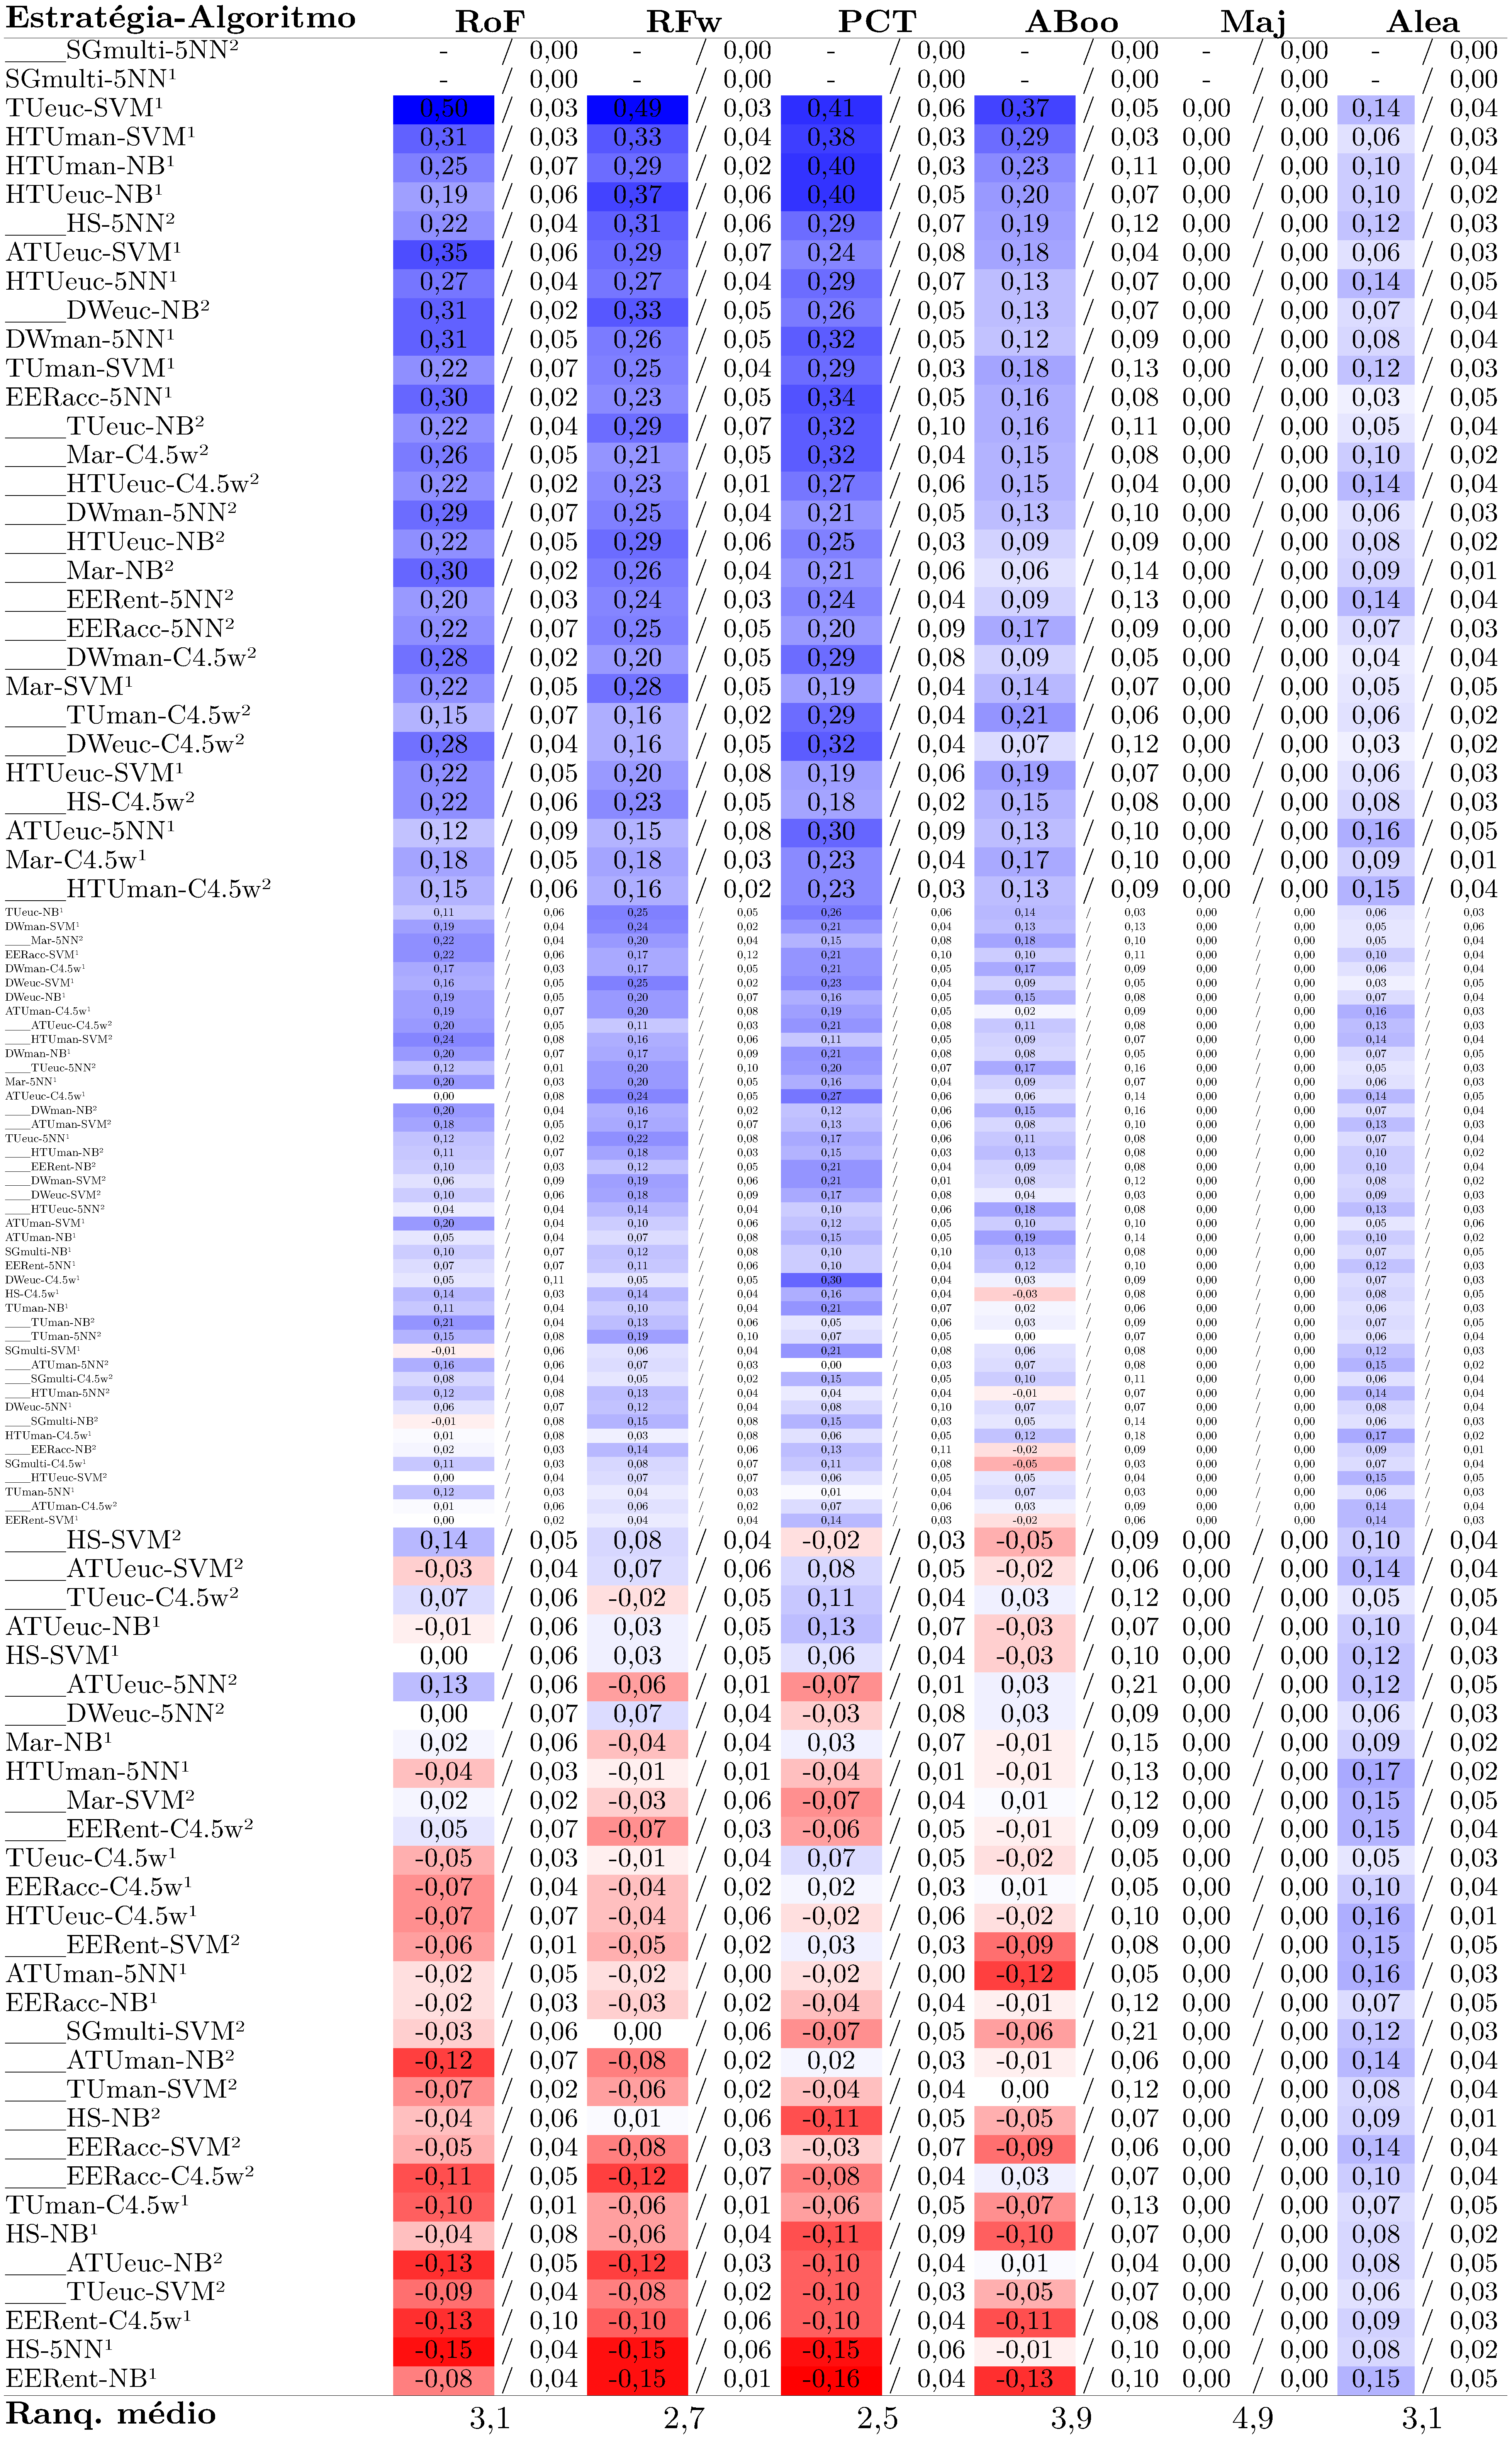
\includegraphics[scale=0.215]{images/metaaa.pdf}
% acc: 10x10-fold
% teste: sem teste
\caption[Comparação de $\kappa$ na recomendação de uso de aprendizado ativo.]{Comparação de $\kappa$ (média/desvio padrão) na recomendação de uso ou não uso de aprendizado ativo.
\textit{A estratégia Rnd foi sempre a melhor opção nas duas primeiras linhas.}
\textit{Detalhes na Figura \ref{accmeta}.}}
\label{aa}
\end{figure}
Apesar desse resultado mostrar que o uso do meta-aprendiz levou a recomendações melhores que %garantir a superação da 
a referência Maj, a referência Alea mostra-se mais segura, por ter apenas valores positivos.
Consequentemente, \destaque{há indícios de que a predição automática da efetividade do aprendizado ativo, para uma dada estratégia e um dado algoritmo de aprendizado \ul{arbitrariamente} definidos, não seja recomendável}.
No entanto, HTU constou 5 vezes entre os 30 experimentos na parte superior da figura e apenas 1 vez entre os 30 experimentos da parte inferior.
Assim, \destaque{há indícios de que a estratégia HTU ofereça maior previsibilidade quanto à possibilidade de predição da efetividade do aprendizado ativo}.

Um ponto importante a ser considerado é que, numa situação real, os pares mais adequados - ou os pares menos adequados - podem ser conhecidos de antemão pelo especialista, determinando quais linhas da Figura \ref{aa} correspondem às necessidades da aplicação.
Essa quantidade reduzida de linhas permitiria saber mais precisamente se a recomendação de uso de aprendizado ativo supera ou não as referências.
